Au départ nous étions parti sur une architecture avec un serveur web qui communiquait avec les clients grâce à des requêtes web HTTP.

Malheureusement cette architecture n'était pas adaptée pour un jeu de ce type puisque au moment où un joueur joue un coup, l'autre joueur doit être notifié de ce changement. Or si on utilise un serveur web HTTP le client devrait faire une requête au serveur pour être mis au courant, ce qui n'est pas pratique.

Pour un changement en direct sans faire une boucle de requêtes continuelles, il faudrait un système où le serveur peut envoyer un message au client sans requête au préalable.

C'est pour cela qu'une architecture avec des web sockets a été la solution que nous avons choisi.
Cette architecture permet d'envoyer des messages ou des données aux clients sans requête préalable.


\begin{figure}[H]
    \centering
    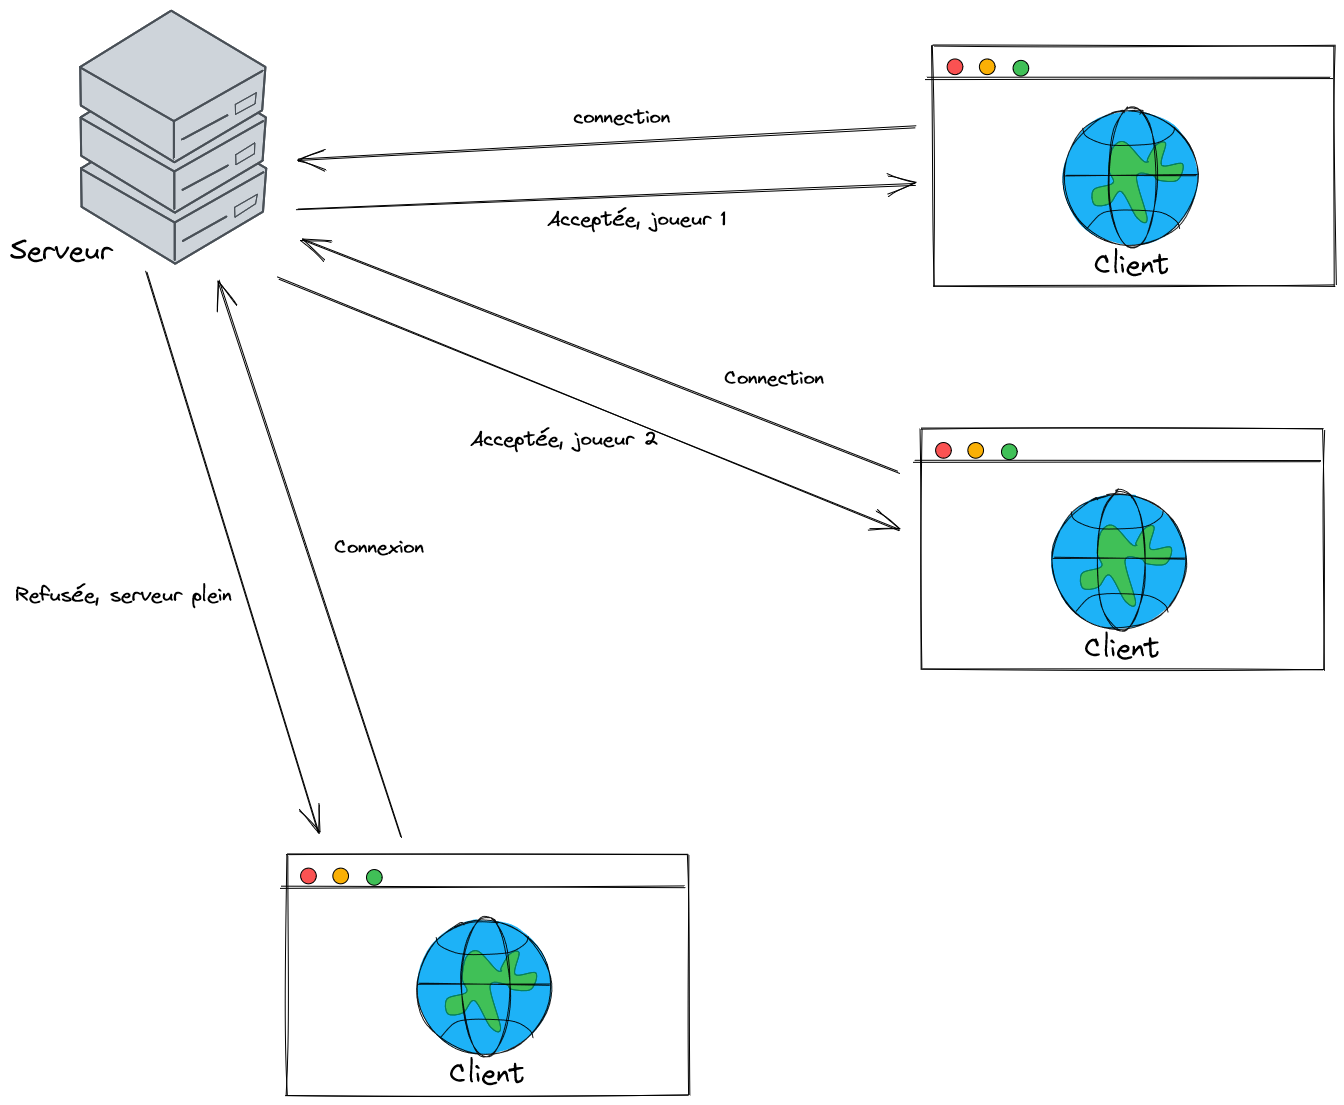
\includegraphics[scale=0.25]{data/reseau_initialisation.png}
    \caption{Phase de connexion des joueurs au serveur}
\end{figure}

Ici on peut voir la première phase du serveur qui permet d'enregistrer les connexions des deux joueurs pour créer une partie.

La partie de connexion est gérée par la bibliothèque {\tt socket-io} que nous utilisons pour le serveur et le client. C'est l'avantage essentiel d'utiliser la même technologie sur le backend et le frontend.

Dans le serveur, nous sauvegardons les sockets qui se connectent au serveur. La limite est de 2 puisqu'il y a 2 joueurs maximum. Quand les 2 joueurs sont bien connectés, la partie est pleine. Si il y en a déjà 2 lors d'une connexion d'une troisième socket, alors la connexion de la troisième est refusée et cette dernière reçoit un code d'erreur, {\tt full}, que le frontend de cette socket va afficher à l'utilisateur.
Si un autre joueur essaie de se connecter, alors la socket n'est pas sauvegardée dans le serveur et elle est déconnectée, il reçoit également une erreur 'full' qui va s'afficher dans le terminal.

Une fois les deux joueurs créé et la partie initilialisée, la carte est envoyée aux deux joueurs pour l'affichage.

Les phases vont donc s'enchaîner jusqu'à ce qu'une action d'un joueur soit requise.

\begin{figure}[H]
    \centering
    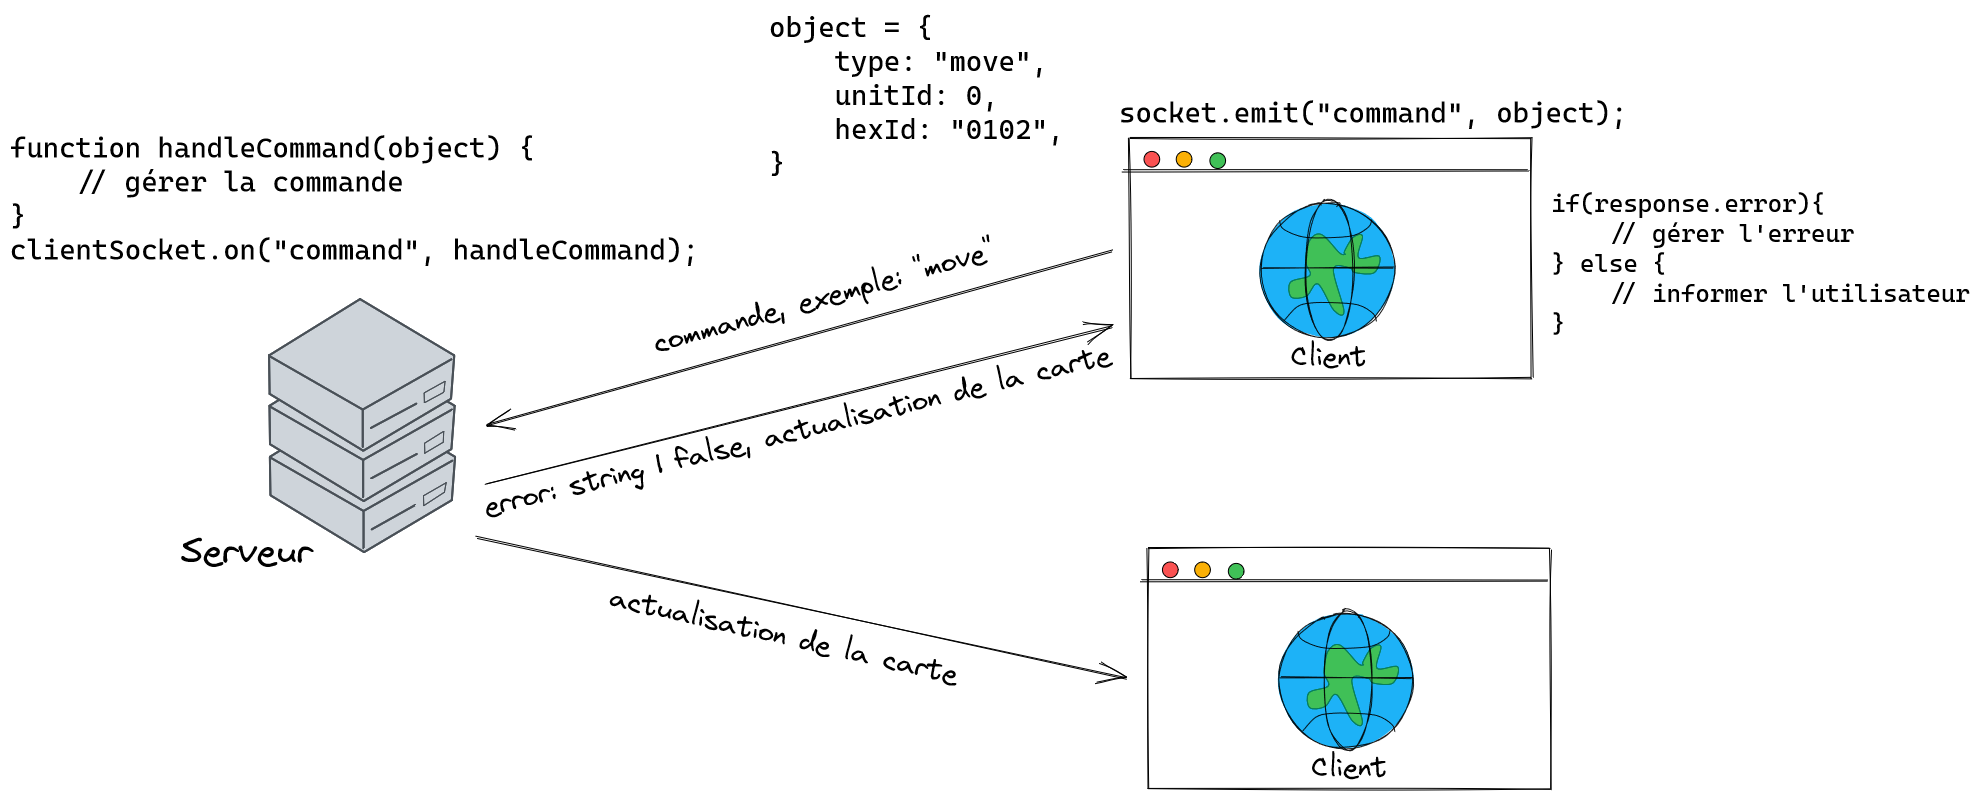
\includegraphics[scale=0.25]{data/reseau_commande.png}
    \caption{Phase de jeu, exemple de commande {\tt move}}
\end{figure}

TODO

La partie s'execute normalement jusqu'à la fin.